\iffalse
\documentclass[journal,10pt,twocolumn]{article}
\usepackage{graphicx}
\usepackage[margin=0.5in]{geometry}
\usepackage[cmex10]{amsmath}
\usepackage{amssymb}
\usepackage{array}
\usepackage{booktabs}
\usepackage{mathtools}
\usepackage{dirtree}
\usepackage{xcolor}
\usepackage{float}
\usepackage[justification=centering,font={rm,md,scriptsize}]{caption}
\usepackage{enumitem}
\usepackage{listings}
\usepackage{mathtools}
\usepackage{fancyvrb}
\usepackage{hyperref}

%Add chapter functionality in IEEEtran class
\newcounter{Chapcounter}
\newcommand\showmycounter{\addtocounter{Chapcounter}{1}\themycounter}
\newcommand{\chapter}[1] 
{ {\centering          
  \addtocounter{Chapcounter}{1} \large \textbf{Chapter \theChapcounter ~#1}}  
  \addcontentsline{toc}{section}{Chapter ~\theChapcounter~~ #1}    
  \setcounter{section}{0}
}
%%%%

\counterwithin{enumi}{section}
\counterwithin{equation}{enumi}
\counterwithin{figure}{enumi}

\renewcommand\thesection{\theChapcounter.\arabic{section}}
%\renewcommand\thesectiondis{\theChapcounter.\arabic{section}}
\newcommand\figref{Fig.~\ref}

\setenumerate{label=\thesection.\arabic*}

\lstset{
  basicstyle=\ttfamily,
  columns=fullflexible,
  frame=single,
  breaklines=true,
  postbreak=\mbox{\textcolor{red}{$\hookrightarrow$}\space},
}

\providecommand{\mbf}{\mathbf}
\providecommand{\pr}[1]{\ensuremath{\Pr\left(#1\right)}}
\providecommand{\qfunc}[1]{\ensuremath{Q\left(#1\right)}}
\providecommand{\sbrak}[1]{\ensuremath{{}\left[#1\right]}}
\providecommand{\lsbrak}[1]{\ensuremath{{}\left[#1\right.}}
\providecommand{\rsbrak}[1]{\ensuremath{{}\left.#1\right]}}
\providecommand{\brak}[1]{\ensuremath{\left(#1\right)}}
\providecommand{\lbrak}[1]{\ensuremath{\left(#1\right.}}
\providecommand{\rbrak}[1]{\ensuremath{\left.#1\right)}}
\providecommand{\cbrak}[1]{\ensuremath{\left\{#1\right\}}}
\providecommand{\lcbrak}[1]{\ensuremath{\left\{#1\right.}}
\providecommand{\rcbrak}[1]{\ensuremath{\left.#1\right\}}}
\newcommand{\sgn}{\mathop{\mathrm{sgn}}}
\providecommand{\abs}[1]{\left\vert#1\right\vert}
\providecommand{\res}[1]{\Res\displaylimits_{#1}} 
\providecommand{\norm}[1]{\left\lVert#1\right\rVert}
\providecommand{\mtx}[1]{\mathbf{#1}}
\providecommand{\mean}[1]{E\left[ #1 \right]}
\providecommand{\fourier}{\overset{\mathcal{F}}{ \rightleftharpoons}}
\providecommand{\ztrans}{\overset{\mathcal{Z}}{ \rightleftharpoons}}
\providecommand{\system}{\overset{\mathcal{H}}{ \longleftrightarrow}}
\newcommand{\solution}{\noindent \textbf{Solution: }}
\newcommand{\cosec}{\,\text{cosec}\,}
\providecommand{\dec}[2]{\ensuremath{\overset{#1}{\underset{#2}{\gtrless}}}}
\newcommand{\myvec}[1]{\ensuremath{\begin{pmatrix}#1\end{pmatrix}}}
\newcommand{\mydet}[1]{\ensuremath{\begin{vmatrix}#1\end{vmatrix}}}
\providecommand{\gauss}[2]{\mathcal{N}\ensuremath{\left(#1,#2\right)}}
\newcommand*{\permcomb}[4][0mu]{{{}^{#3}\mkern#1#2_{#4}}}
\newcommand*{\perm}[1][-3mu]{\permcomb[#1]{P}}
\newcommand*{\comb}[1][-1mu]{\permcomb[#1]{C}}

\let\vec\mathbf

\def\putbox#1#2#3{\makebox[0in][l]{\makebox[#1][l]{}\raisebox{\baselineskip}[0in][0in]{\raisebox{#2}[0in][0in]{#3}}}}
     \def\rightbox#1{\makebox[0in][r]{#1}}
     \def\centbox#1{\makebox[0in]{#1}}
     \def\topbox#1{\raisebox{-\baselineskip}[0in][0in]{#1}}
     \def\midbox#1{\raisebox{-0.5\baselineskip}[0in][0in]{#1}}

\begin{document}

\title{Transformation of Random Variables}
\author{Sampath Govardhan}

\maketitle

\tableofcontents

\bigskip

\fi

\section{Gaussian to Other}

\begin{enumerate}

\item
Let $X_1 \sim  \gauss{0}{1}$ and $X_2 \sim  \gauss{0}{1}$. Plot the CDF and PDF of
%
\begin{equation}
V = X_1^2 + X_2^2
\end{equation}\\
\solution The CDF and PDF of $V$ are plotted in \figref{fig:chisq_cdf} and \figref{fig:chisq_pdf} respectively using the below code
\begin{lstlisting}
codes/ch4_squares.py
\end{lstlisting}
\begin{figure}[h]
\centering
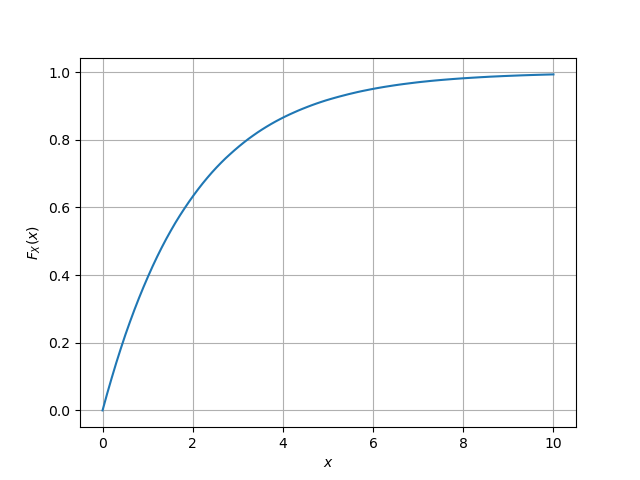
\includegraphics[width=\columnwidth]{./chapters/ch4/figs/ch4_squarescdf.png}
\caption{CDF of $V$}
\label{fig:chisq_cdf}
\end{figure}
\begin{figure}[h]
\centering
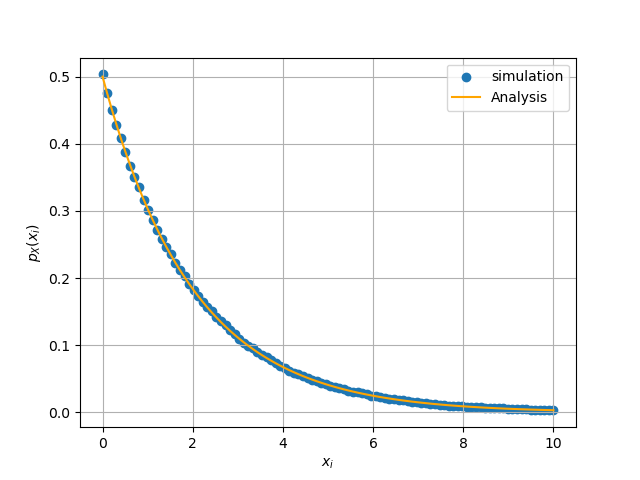
\includegraphics[width=\columnwidth]{./chapters/ch4/figs/ch4_squarespdf.png}
\caption{PDF of $V$}
\label{fig:chisq_pdf}
\end{figure}
%

%
%
\item
If
%
\begin{equation}
F_{V}(x) = 
\begin{cases}
1 - e^{-\alpha x} & x \geq 0 \\
0 & x < 0,
\end{cases}
\label{eq:chisq2_cdf_gen}
\end{equation}
%
find $\alpha$.\\
\solution Let $Z=X^2$ where $X \sim \gauss{0}{1}$. Defining the CDF for $Z$,
\begin{flalign*}
	P_Z(z) &= \pr{Z < z}&\\
	&= \pr{X^2 < z}&\\
	&= \pr{-\sqrt{z} < X < \sqrt{z}}&\\
	&= \int_{-\sqrt{z}}^{\sqrt{z}} p_X(x)  \,dx 
\end{flalign*}
Using \eqref{eq:cdf_to_pdf}, the PDF of $Z$ is given by
\begin{align}
	\nonumber
	\frac{d}{dz}P_Z(z) &= p_Z(z)\\
	\label{eq:square_pdf_gen}
	= \frac{p_X(\sqrt{z})+p_X(-\sqrt{z})}{2\sqrt{z}} & \text{ (Using Lebniz's rule)} 
\end{align}
Substituting the standard gaussian density function $p_X(x) = \frac{1}{\sqrt{2\pi}}e^{-\frac{x^2}{2}}$ in \eqref{eq:square_pdf_gen},
\begin{equation}
	p_Z(z) =
	\begin{cases}
	\frac{1}{\sqrt{2\pi z}}e^{-\frac{z}{2}} & z \ge 0\\
	0 & z < 0
	\end{cases} 
	\label{eq:chisq_pdf}
\end{equation}
The PDF of $X_1^2$ and $X_2^2$ are given by \eqref{eq:chisq_pdf}. Since $V$ is the sum of two independant random variables,
\begin{flalign*}
	p_V(v) &= p_{X_1^2}(x_1) \ast p_{X_2^2}(x_2)&\\
	&= \frac{1}{2\pi} \int_{0}^{v} \frac{e^{-\frac{x}{2}}}{\sqrt{x}}\frac{e^{-\frac{v-x}{2}}}{\sqrt{v-x}}  \,dx&\\
	&= \frac{e^{-\frac{v}{2}}}{2\pi} \int_{0}^{v} \frac{1}{\sqrt{x(v-x)}}  \,dx&\\
	&= \frac{e^{-\frac{v}{2}}}{2\pi} \sbrak{-\arcsin\left(\dfrac{v-2x}{v}\right)}_0^v&\\
	&= \frac{e^{-\frac{v}{2}}}{2\pi} \pi&\\
	&= \frac{e^{-\frac{v}{2}}}{2} \text{ for } v \ge 0
\end{flalign*}
$F_V(v)$ can be obtained from $p_V(v)$ using \eqref{eq:pdf_to_cdf}
\begin{flalign}
	\nonumber
	F_V(v) &= \frac{1}{2} \int_{0}^{v} \exp\left(-\frac{v}{2}\right)&\\
	\label{eq:chisq2_cdf}
	&= 1-\exp\left(-\frac{v}{2}\right) \text{ for } v \ge 0
\end{flalign}
Comparing \eqref{eq:chisq2_cdf} with \eqref{eq:chisq2_cdf_gen}, $\alpha = \frac{1}{2}$ 
%
\item
\label{ch3_raleigh_sim}
Plot the CDF and PDF of
%
\begin{equation}
A = \sqrt{V}
\end{equation}\\
\solution The CDF and PDF of $A$ are plotted in $$\figref{fig:rayleigh_cdf}$$ and $$\figref{fig:rayleigh_pdf}$$ respectively using the below code
\begin{lstlisting}
codes/ch4_sqrt.py
\end{lstlisting}
The CDF of $A$ is given by,
\begin{align}
	F_{A}\brak{a} &= \pr{A < a}\\
	&= \pr{\sqrt{V} < a}\\
	&= \pr{V < a^2}\\
	&= F_{V}\brak{a^2}\\
	&= 1-\exp\brak{-\frac{a^2}{2}} 
\end{align}
Using \eqref{eq:cdf_to_pdf}, the PDF is found to be
\begin{align}
	p_{A}\brak{a} &= a\exp\brak{-\frac{a^2}{2}}
\end{align}
\begin{figure}[h]
\centering
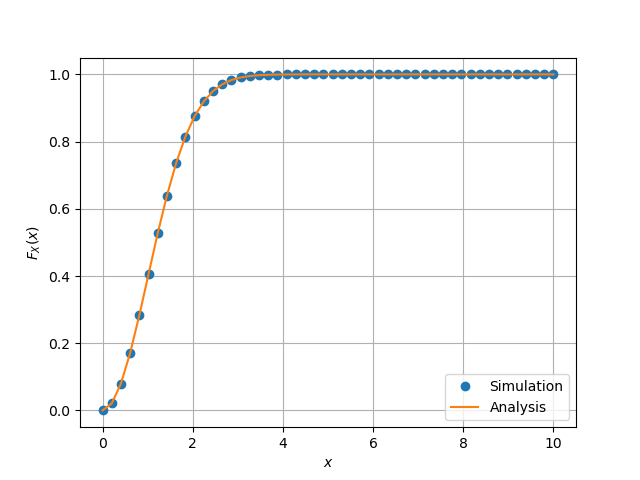
\includegraphics[width=\columnwidth]{./chapters/ch4/figs/ch4_sqrtcdf.png}
\caption{CDF of $A$}
\label{fig:rayleigh_cdf}
\end{figure}
\begin{figure}[h]
\centering
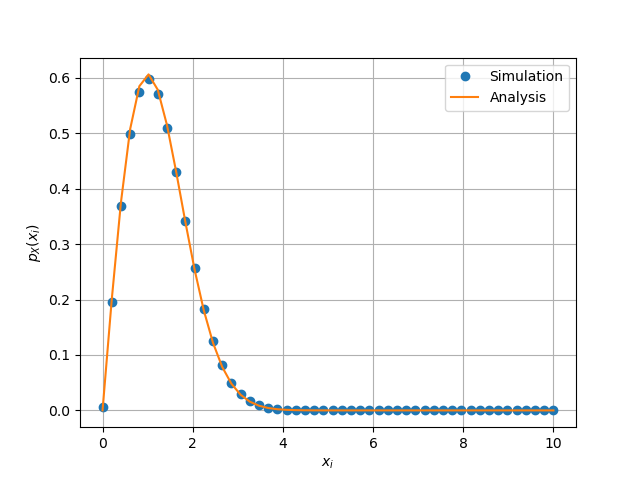
\includegraphics[width=\columnwidth]{./chapters/ch4/figs/ch4_sqrtpdf.png}
\caption{PDF of $A$}
\label{fig:rayleigh_pdf}
\end{figure}
%


\end{enumerate}

\section{Conditional Probability}
\begin{enumerate}
\item
\label{ch4_sim}
Plot 
\begin{equation}
P_e = \pr{\hat{X} = -1|X=1}
\end{equation}
%
for 
\begin{equation}
Y = AX+N,
\end{equation}
where $A$ is Raleigh with $E\sbrak{A^2} = \gamma, N \sim \gauss{0}{1}, X \in \brak{-1,1}$ for $0 \le \gamma \le 10$ dB.\\
\solution The blue dots in \figref{fig:bpsk_pe_snr_rayleigh} is the required plot. The below code is used to generate the plot,
\begin{lstlisting}
codes/ch4/ch4_err.py
\end{lstlisting}
%
\item
Assuming that $N$ is a constant, find an expression for $P_e$.  Call this $P_e(N)$\\
\solution Assuming the decision rule in \eqref{eq:bpsk_decision}, when $N$ is constant, $P_e$ is given by 
\begin{flalign}
	\nonumber
	P_e &= \pr{\hat{X} = -1|X=1}&\\ \nonumber
	&= \pr{Y<0|X=1}&\\ \nonumber
	&= \pr{AX+N<0|X=1}&\\ 
	\label{eq:prob_err_rayleigh_gen}
	&= \pr{A+N<0}&\\ \nonumber
	&= \pr{A<-N}&\\
	\label{eq:prob_err_bpsk_rayleigh_cdf}
	&=
	\begin{cases}
	F_A(-N) & N \ge 0\\
	0 & N < 0
	\end{cases}
\end{flalign}
For a Rayleigh random variable $X$ with $E\sbrak{X^2} = \gamma$, the PDF and CDF are given by
\begin{align}
	\label{eq:rayleigh_pdf}
	p_X(x) &= \frac{2x}{\gamma}\exp\left(-\frac{x^2}{\gamma}\right) \text{ for } x \ge 0\\
	\label{eq:rayleigh_cdf}
	F_X(X) &= 1-\exp\left(-\frac{x^2}{\gamma}\right) \text{ for } x \ge 0
\end{align}
Substituting \eqref{eq:rayleigh_cdf} in \eqref{eq:prob_err_bpsk_rayleigh_cdf},
\begin{equation}
	\label{eq:prob_err_bpsk_rayleigh_fN}
	P_e(N) =
	\begin{cases} 
	1-\exp\left(-\frac{N^2}{\gamma}\right) & N \ge 0\\
	0 & N < 0
	\end{cases}
\end{equation}
%
\item
%
\label{ch4_anal}
For a function $g$,
\begin{equation}
E\sbrak{g(X)} = \int_{-\infty}^{\infty}g(x)p_{X}(x)\, dx
\end{equation}
%
Find $P_e = E\sbrak{P_e(N)}$.\\
\solution Using $P_e(N)$ from \eqref{eq:prob_err_bpsk_rayleigh_fN},
\begin{flalign*}
	P_e &= \int_{-\infty}^{\infty} P_e(x)p_N(x) \,dx&\\
	&= \int_{0}^{\infty} \left(1-e^{-\frac{x^2}{\gamma}}\right)\frac{1}{\sqrt{2\pi}}e^{-\frac{x^2}{2}} \,dx
\end{flalign*}
	
\begin{multline*}
	P_e = \frac{1}{\sqrt{2\pi}}\int_{0}^{\infty} e^{-\frac{x^2}{2}}  \,dx \\ - \frac{1}{\sqrt{2\pi}}\int_{0}^{\infty} \exp\left(-x^2\left(\frac{1}{\gamma}+\frac{1}{2}\right)\right)  \,dx
\end{multline*}
\begin{flalign*}
	P_e &= \frac{1}{2} - \frac{1}{2}\sqrt{\frac{\gamma}{2+\gamma}}
\end{flalign*} 
%
\item
Plot $P_e$ in problems \ref{ch4_sim} and \ref{ch4_anal} on the same graph w.r.t $\gamma$.  Comment.\\
\solution $P_e$ plotted in same graph in \figref{fig:bpsk_pe_snr_rayleigh}. The value of $P_e$ is much higher when the channel %
gain $A$ is Rayleigh distributed than the case where $A$ is a constant (compare with \figref{fig:bpsk_pe_snr}).
\begin{figure}[H]
\centering
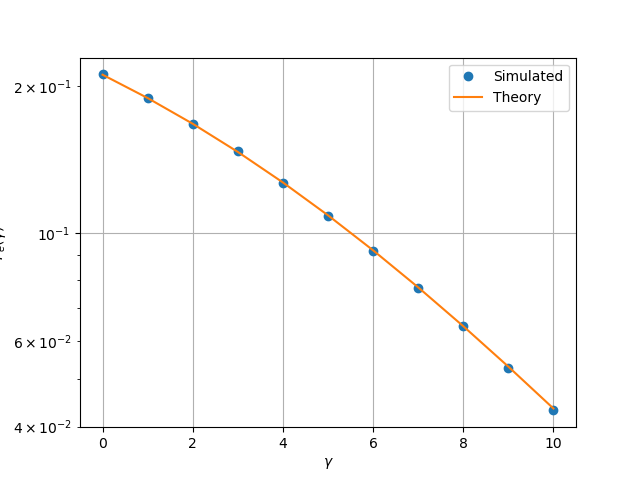
\includegraphics[width=\columnwidth]{./chapters/ch4/figs/ch4_error.png}
\caption{$P_e$ versus $\gamma$}
\label{fig:bpsk_pe_snr_rayleigh}
\end{figure}
From \eqref{eq:prob_err_rayleigh_gen}, $P_e$ is given by
\begin{equation}
	P_e = \pr{A+N<0}
\end{equation}
One method of computing \eqref{eq:prob_err_rayleigh_gen} is by finding the PDF of $Z=A+N$ (as the convolution of the individual PDFs of %
$A$ and $N$) and then integrating $p_Z(z)$ from $-\infty$ to $0$. The other method is by first computing $P_e$ for constant $N$ and then finding %
the expectation of $P_e(N)$. Both provide the same result but the computation of integrals is simpler when using the latter method. 

\end{enumerate}

%\end{document}
